\documentclass{article}
\usepackage{graphicx}
\usepackage{float}
\usepackage{subcaption}
\usepackage{natbib}
\usepackage{indentfirst}
\usepackage{chngcntr}
\usepackage[a4paper]{geometry}
\usepackage{fancyhdr}
\usepackage[hidelinks]{hyperref}
\usepackage{mathrsfs}
\usepackage[toc,page]{appendix}
\usepackage{csquotes}
\usepackage[longtable]{multirow}
\usepackage{longtable}
\usepackage{booktabs} % Para tablas súper pro
\usepackage{vcell}
\usepackage{array}
\usepackage{epsfig}
\usepackage{pdfpages}
\usepackage{amssymb}
\usepackage{pmboxdraw}
\usepackage{alltt}
\usepackage{listings}
\usepackage{listingsutf8}
%\usepackage[spanish, es-tabla]{babel} % Para que ponga tabla en vez de cuadro
\usepackage{xcolor}
\usepackage{url}
\usepackage{svg}
\usepackage{xcolor,colortbl, pifont}
\usepackage{booktabs}
\usepackage{gensymb}
\usepackage{dirtytalk}
\usepackage{cancel} % Para tachar términos de ecuaciones
\usepackage{siunitx}
\usepackage{mathtools}
\usepackage{empheq}
\usepackage{titlesec}



\lstset{
     literate=%
         {á}{{\'a}}1
         {í}{{\'i}}1
         {é}{{\'e}}1
         {ú}{{\'u}}1
         {ó}{{\'o}}1
         {Á}{{\'A}}1
         {Í}{{\'I}}1
         {É}{{\'E}}1
         {Ú}{{\'U}}1
         {Ó}{{\'O}}1}

\definecolor{codegreen}{rgb}{0,0.6,0}
\definecolor{codegray}{rgb}{0.5,0.5,0.5}
\definecolor{codepurple}{rgb}{0.58,0,0.82}
\definecolor{backcolour}{rgb}{0.95,0.95,0.92}

\lstdefinestyle{mystyle}{
    backgroundcolor=\color{backcolour},   
    commentstyle=\color{codegreen},
    keywordstyle=\color{magenta},
    numberstyle=\tiny\color{codegray},
    stringstyle=\color{codepurple},
    basicstyle=\ttfamily\footnotesize,
    breakatwhitespace=false,         
    breaklines=true,                 
    captionpos=b,                    
    keepspaces=true,                 
    numbers=left,                    
    numbersep=5pt,                  
    showspaces=false,                
    showstringspaces=false,
    showtabs=false,                  
    tabsize=2
}
\lstset{style=mystyle}


\numberwithin{equation}{section}
\numberwithin{equation}{subsection}
\counterwithin{figure}{section}
\counterwithin{table}{section}
\AtBeginDocument{\counterwithin{lstlisting}{section}}
%
% \renewcommand{\thesection}{Sección \Arabic{section}}

% \renewcommand{\figureautorefname}{Figura}
% \renewcommand{\tableautorefname}{Tabla}
% \renewcommand{\equationautorefname}{Ecuación}

\newcommand*\colourcheck[1]{%
  \expandafter\newcommand\csname #1check\endcsname{\textcolor{#1}{\ding{52}}}%
}
\colourcheck{blue}
\colourcheck{green}
\colourcheck{red}


\geometry{top=3.5cm, bottom=3.5cm, left=3cm, right=3cm}

\pagestyle{fancy}
\fancyhf{}
\lhead{MUSE: Integración y Ensayos}
\rhead{
\includegraphics[height=0.8cm]{Images Document/logomuse2.png}} % right logo
\cfoot{\thepage}



\begin{document}

\begin{center}
    \thispagestyle{empty}

    
\includegraphics[width=16.5cm]{Images Document/Logo_portada.png} \\

    \vspace{1cm}

    \Large{Universidad Politécnica de Madrid \\
        \vspace{0.35cm}
        Escuela Técnica Superior de Ingeniería Aeronáutica y del Espacio \\
        \vspace{0.35cm}
        Máster Universitario en Sistemas Espaciales \\}

    \begin{center}
        \vspace{2 cm}
        {\bfseries\Huge Mejora de simulador y analisis de viabilidad de misiones espaciales dedicadas a Space Situational Awareness (SSA) \\}
        \vspace{1 cm}
        \textbf{Caso de estudio 2 \\}
        \vspace{0.5cm}

        {\large{\textbf{\today}}}

        \vfill
        {\Large Autora: \\
            Inés Arauzo Andrés \\
        }


    \end{center}
\end{center}

\pagenumbering{gobble}
\thispagestyle{empty}

\newpage
\pagenumbering{Roman} % Numeración romana hasta la primera sección


\tableofcontents


\setlength{\parskip}{4mm}
\setlength{\parindent}{20pt}
\setlength{\headheight}{16.07225pt}

\newpage
\pagenumbering{arabic}


\section{Introduction}
The continuous growth in the number of objets (active satellites and space debris) has significantly raised the probability of collisions, endangering the safety of spacecrafts and satellite constellations. Hence, in order to ensure the safety and organization of activities in space, it has become crutial to quickly develop and enhance Space Situational Awareness (\textit{SSA}).


\begin{figure}[ht]
    \centering
    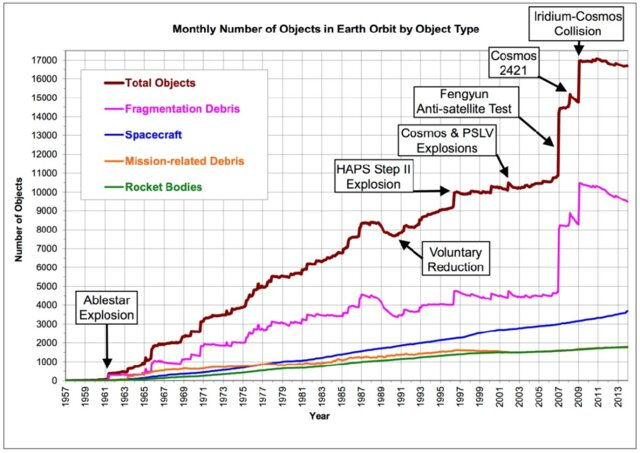
\includegraphics[width=0.8\columnwidth]{Figures/Growth-of-orbital-space-object-including-space-debris-NASA-Orbital-Debris-program_W640.jpg}
    \caption{Timeline of orbital space debris growth.}
    \label{fig:orbital_debris_growth}
\end{figure}

In this context, \textit{SSA}, which is defined as the knowledge and characterization of space objects and their operational environment, has evolved into a pivotal solution  to mitigate the growing hazards in space. While terrestrial \textit{SSA} has worked as the foundational framework, the dynamic evolution of the space environment needs a paradigm shift towards space-centric \textit{SSA}. This strategic transition entails considerable advantages in precision, operational efficiency, and system stability as compared to its terrestrial counterpart.


The area under surveillance now extends from low Earth orbits (LEO) to a terrestrial radius of at least 100,000 km. This broader coverage essentially includes all objects in orbit, encompassing both artificial and natural entities that may pose potential risks. However, there is a remarkable interest in the Low Earth Orbits due to the increasing density of satellite deployments and space activities within this region.

With the objective of  reaching the desired scope of monitoring, the adoption of advanced remote sensing and continuous monitoring technologies  has been proved essential. These technologies enable the precise identification and analysis of space threats, including debris and asteroids, contributing to a strong and proactive \textit{SSA}.


In this context, there is an imperative need for the development of specialized simulators tailored to the precise detection and tracking of space debris. These simulators must be able to provide a faithful representation of the space environment, allowing  the training and validation of \textit{SSA} strategies to work.


Space Situational Awareness, particularly in the realm of debris detection and tracking, stands as a critical component for space safety and sustainability. The adoption of advanced technologies, the transition to space-based \textit{SSA}, and the development of specialized simulators are essential steps toward the effective management of risks in orbit.

In conclusion, the increasing challenges arising from the growing number of objects in space underscore the need for a comprehensive approach to Space Situational Awareness (SSA). To address this issue, the integration of advanced technologies and the development of specialized simulators become pivotal elements. These measures collectively play a crucial role in ensuring the safety and sustainability of activities within Earth's orbit. By combining cutting-edge technologies with purpose-built simulators, we can effectively navigate the evolving complexities associated with managing risks in space.


\subsection{Motivación para Mejorar el Simulador de \textit{SSA}}

Recognizing the urgent need to systematically register and locate space debris, an initial version of a Space Situational Awareness (SSA) simulator was developed. This simulator, characterized by a basic design and a notably disorganized code structure (explained in Section \ref{s: Code}), is being requested for improvement to achieve preliminary results.

The main motivation for enhancing the SSA simulator comes from the necessity to integrate a specialized photometry module. Photometry, which involves precise measurements of light emitted by celestial entities, is of utmost importance for the detailed characterization of space debris. The addition of this module is expected to enable a more accurate simulation of the visual attributes of celestial objects in space, thereby strengthening the simulator's capacity to faithfully replicate real-world conditions.

In the process of integrating the new photometry module, the primary objective is to determine the effective range of the sensors. This step is pivotal as it serves as the foundation for the development of essential positioning functions. By accurately establishing the sensor range, these functions will facilitate the strategic positioning of observers in specific orbits. The goal is to ensure optimal visibility of the target by a minimum of 1 observer. This meticulous approach not only enhances the simulator's spatial accuracy but also improves its ability to replicate real-world observational scenarios with greater precision.

Moreover, when considering the evaluation of simulator accuracy, the focus extends beyond a general assessment based on observer numbers and average visibility times. The intention is to delve into the intricate interplay between these factors, seeking to identify patterns and dependencies that may impact the simulator's predictive capabilities. Through an analysis of how the simulator responds to variations in observer counts and average visibility times, valuable insights into the subtleties of its performance under diverse conditions can be obtained. This comprehensive examination is indispensable for validating the simulator's effectiveness in providing reliable space situational awareness, thereby establishing a robust foundation for advancements in the understanding and monitoring of space debris.



\newpage
\section{Code development}\label{s: Code}
\subsection{Code Refactoring for Improved Modularity in a Space-Based SSA Simulator}
As discussed in the introduction, the initial codebase of the simulator comprised a single folder containing a highly extensive main code. This code encompassed simulation parameters, the structure and parameters of the estimator, simulation errors, and other essential components. Within this folder, there were some other functions used by the main program and another subfolder housing the simulation program itself, invoked from the main program. In essence, the initial simulator had been developed following a spaghetti-code philosophy, lacking a structured approach that would facilitate both code comprehension and the implementation of potential enhancements.

Motivated by the need for a more organized and maintainable codebase, a decision was made to refactor the code into modules, adhering to an imperative programming paradigm. This restructuring aimed to enhance code readability and facilitate the subsequent implementation of various functions and modules, providing a foundation for future improvements.

The refactoring process involved the systematic division of the monolithic code into distinct modules, each addressing specific functionalities or components of the simulator. This modular approach not only promotes code clarity but also streamlines the integration of new features and the maintenance of existing ones.

The refactored code now embraces a more modular and organized structure, aligning with best practices in software engineering. This restructuring sets the stage for further advancements and improvements in the space-based Space Situational Awareness (SSA) simulator, fostering a more sustainable and extensible development process.

The restructured code now features a main code accessed through a more user-friendly interface (\textit{SimConfig.m}). The code is organized into several modules residing in subfolders:

\begin{itemize}
    \item \textbf{Estimation Module:} This module houses functions employed as estimators. Currently, the sole proposed estimator is the Unscented Kalman Filter (UKF) which implies several functions. However, any additional estimators introduced in the future would find their place within this module.

    \item \textbf{Physics Module:} This module contains functions that mathematically represent the physics of the problem intended for simulation. It encompasses aspects such as orbit propagation, solar ephemerides, and other relevant physical phenomena.

    \item \textbf{Simulation Module:} The core simulation code (\textit{Data\_Simulation.m}) resides in this module, along with the code responsible for generating the desired type of satellite (\textit{Satellite.m}).

    \item \textbf{Photometry Module:} This module incorporates functions developed in Section \ref{s: fotometria}, addressing photometric considerations within the simulation.

    \item \textbf{Utilities Module:} Essential functions for the proper execution of the program are stored here. These include functions for coordinate transformations, quaternion-to-rotation matrix conversions, and other utility functions.
\end{itemize}

This modular organization enhances code manageability, readability, and extensibility. It establishes a clear separation of concerns, allowing for straightforward integration of new functionalities and easing the maintenance process. The user-friendly entry point (\textit{SimConfig.m}) serves as a central interface, providing a more intuitive and accessible means to configure and run the simulator.

\subsection{Program Workflow and Execution Sequence}
As discussed earlier, the program operation unfolds through two primary components: the simulator and the estimator. These modules sequentially execute upon being invoked from the main program, where the main parameters of the simulation are introduced, as defined in \textit{Sim\_config.m}. These parameters encompass the dimensions, attitude, and initial position of the target debris, observer number and altitude, as well as other simulation parameters such as duration and start date. The following code excerpt illustrates the parameters fed into the main program:


\begin{lstlisting}[language=Matlab, caption= Parameters introduced into the \textit{Main\_Program.m} through \textit{Sim\_config.m}.]
    % Global Constants
    mu=3.986044418e14;
    Rt = 6878000;
    
    % Debris Parameters
    sim_params.sat_size = 2;   
    sim_params.sub_cat = 3;    
    sim_params.deploy_panels = 0;   
    sim_params.rt_init = [500, 0, 0]*1000 + Rt;
    sim_params.qt = [-0.401437297624753;-0.578215887659600;0.239454457519217;0.668712229668289];
    
    % 7Observers Parameters
    sim_params.n_observers = 5;  %
    sim_params.d_1stObs_target = 200000;
    sim_params.ro_init = [750, 0, 0] * 1000 + Rt;
    
    % Simulation Parameters
    sim_params.total_sim_time = 2*pi*sqrt(sim_params.ro_init(1)^3/mu);   
    sim_params.Year = 2023;
    sim_params.Month = 2;
    sim_params.Day = 25;
    sim_params.Hour = 15;
    sim_params.Min = 0;
    sim_params.Sec = 1;
\end{lstlisting}



\subsubsection{Simulation Algorithm}
Upon the invocation of the simulator (\textit{Data\_Simulation.m}), the pre-established parameters, coupled with the defined simulation time steps are incorporated to the simulation workspace. The "\textit{Debris Parameters}" defined in the code above, are used as an input to a MATLAB predefined function named "Satellite" that defines the target as a satellite of the desired dimensions. Subsequently, leveraging the target's position and observer data, two functions are employed to position the observers in orbital locations conducive to observing the target.

The strategic decision was made to position all observers initially in a shared coplanar orbit with the target, visually represented in  \autoref{fig: orbitas-coplanarias}. This aligns with the constellation structure outlined in \cite{constellations}, optimizing the observational efficiency of the network. To define this configuration, two distinct positioning functions were developed.
\begin{figure}[H]
\centering
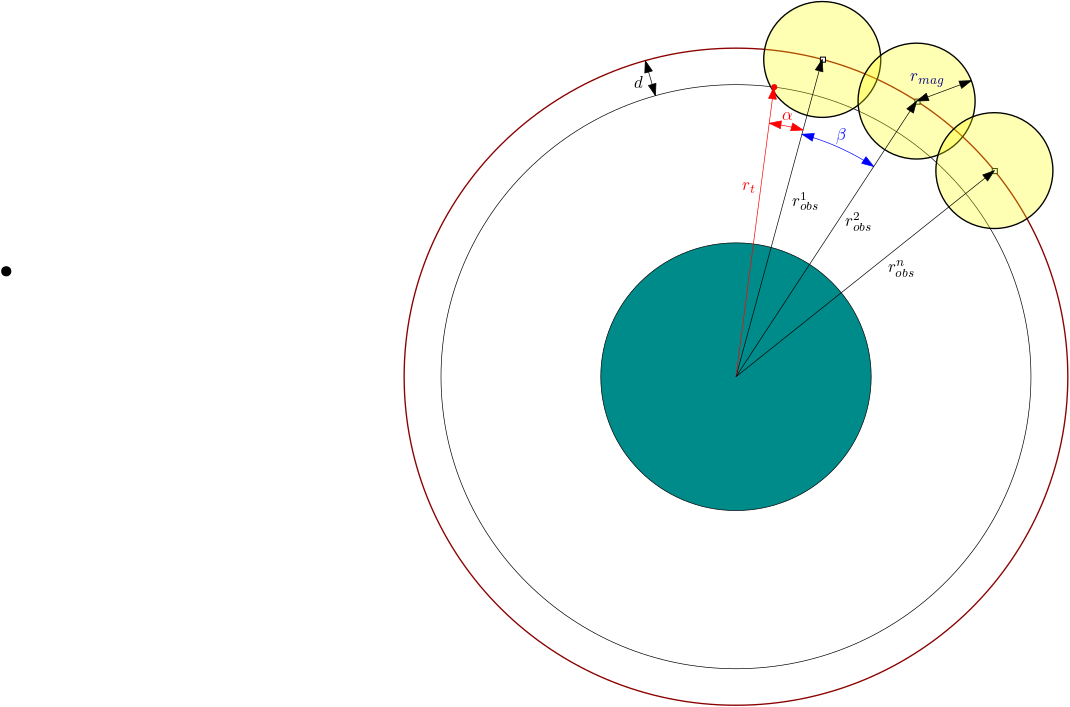
\includegraphics[width=0.6\columnwidth]{Figures/orbitas.png}
\caption{Observers and target orbits configuration}
\label{fig: orbitas-coplanarias}
\end{figure}
The first of these functions, namely \textit{generate\_position\_1st\_obs.m}, takes the lead in constructing the first observer initial position within the specified orbit, drawing parameters from the configuration file. The observer is placed at an angular distance denoted as $\alpha$ from the target.

Afterwards, a complementary function, \textit{generate\_position\_N\_obs.m}, was conceptualized to handle the placement of the remaining observers within the same orbit. This function defines an angular separation denoted as $\beta$ between the observers. It is worth emphasizing that both $\alpha$ and $\beta$ distances are inherently linked to the observer's effective sensor range, defined in the simulation as the radius of the visibility sphere.

It is crucial to highlight that the developed functions are designed to provide both Above the Horizon (ATH) and Below the Horizon (BTH) coverage, as elucidated in \cite{ATH-BTH}. The distinction in positioning arises from the observer's orbital semi-major axis concerning that of the target. When the observer is in an orbit with a semi-major axis greater than that of the target, it will exhibit a lower orbital velocity. To extend the observation time, the observers are strategically positioned with a true anomaly ($\nu$) greater than that of the target, given by $\nu_{obs_1} = \nu_t + \alpha$. Conversely, when the observer is in a lower orbit (providing ATH coverage), it will have a higher orbital velocity. To maximize the observation window in this scenario, the observers are situated with a true anomaly given by $\nu_{obs_1} = \nu_t - \alpha$. This strategic placement ensures comprehensive coverage by adapting to the inherent differences in orbital dynamics.

The nuanced approach to observer positioning becomes evident in the following code snippet:

\begin{lstlisting}[language=Matlab, caption= Excerpt of function \textit{generate\_position\_1st\_obs.m}.]
    function [r, v] = generate_1st_obs_pos(rt, vt, d)
    % Initialize output arrays
    r = zeros(3, 1);
    v = zeros(3, 1);

    % Extract Keplerian elements from the target state vectors
    [a_t, ecc_t, inc_t, RAAN_t, argp_t, nu_t] = ijk2keplerian(rt, vt);

    % Constants, define as wanted
    radius_coverage_sph = 1000000; % [m]this is a function of the magnitude
    initial_offset_o1_t = 10000;

    % Compute adjusted semi-major axis for observers
    a_obs = a_t + d;

    % Compute initial angular offset between the target and the first
    % observer
    alpha = acosd((a_obs^2 + a_t^2 - initial_offset_o1_t^2) / (2 * a_obs * a_t));
    if ~isreal(alpha)
        alpha = 0;
    else
        alpha = mod(alpha, 360);
    end
    % Determine true anomaly for observer 1, with the offset stated
    % previously
    if a_obs > a_t
        nu_obs1 = mod(nu_t + alpha, 360);
    else
        nu_obs1 = mod(nu_t - alpha, 360);
    end

    % Convert observer 1's Keplerian elements to Cartesian coordinates
    [r, v] = keplerian2ijk(a_obs, ecc_t, inc_t, RAAN_t, argp_t, nu_obs1);
end
\end{lstlisting}

The simulation workflow continues by propagating the initial positions of both the observers and the target along their respective orbits, leveraging the Keplerian orbit equation,
\begin{equation}
    \label{eq:state}
    \left\{\begin{aligned}\dot{x}\\\dot{y}\\\dot{z}\\\ddot{x}\\\ddot{y}\\\ddot{z}\end{aligned}\right\}=\left\{\begin{aligned}\dot{\boldsymbol{r}}&\\-\frac{\mu}{r^3}\boldsymbol{r}&+a_p\end{aligned}\right\}.
\end{equation}


In this particular case, the consideration of acceleration attributable to perturbations, denoted as $a_p$, has not been directly incorporated into the analysis. Rather, the introduced noise has been conceptualized as a surrogate for perturbations in the system.

The numerical Runge-Kutta 4 scheme is employed to ensure accurate and stable propagation, as given by the following equations:
\begin{equation}
    \begin{aligned}
        &X_{n+1} =X_n+\frac {\Delta t}{6}\left(k_1+2k_2+2k_3+k_4\right),  \\
        &t_{n+1} =t_n+\Delta t , \quad, with n=0, 1, 2, 3...,\\
    \end{aligned}
\end{equation}
where $X = (x, y, z,\dot{x}, \dot{y},\dot{z})$ represents the state vector, which comprises the position $r=(x, y, z)^T$ and the velocity $v=(\dot{x}, \dot{y},\dot{z})$ , $t$ denotes time, and $k_1, k_2, k_3,$ and $k_4$ are intermediary values calculated as per the Runge-Kutta method,\\
\begin{equation}
    \begin{aligned}
        &k_{1} =f(t_{n},X_{n}),  \\
        &k_{2} =f\biggl(t_{n}+\frac{\Delta t}{2},X_{n}+\Delta t\frac{k_{1}}{2}\biggr),  \\
        &k_{3} =f\biggl(t_{n}+\frac{\Delta t}{2},X_{n}+\Delta t\frac{k_{2}}{2}\biggr),  \\
        &k _4=f(t_{n}+\Delta t,y_{n}+\Delta tk_{3}). \\
        \end{aligned}
\end{equation}
After propagating the orbits, a controlled positioning error, alongside attitude and directional errors, is introduced to the observer. This step is crucial for simulating potential deviations in the measurements that may arise from real-world scenarios. The introduced errors follow a bounded distribution, ensuring a realistic yet manageable level of uncertainty.
Both the perturbed and unperturbed datasets are stored as outputs of the simulator. 

\subsubsection{Estimator Algorithm: Unscented Kalman Filter}


As highlighted in the introduction, a fundamental achievement of Space Situational Awareness (SSA) systems revolves around the determination of Resident Space Object (RSO) size and position. This estimation, often articulated through Keplerian parameters, Cartesian coordinates, or alternative representations, plays a pivotal role in predicting the RSO's future position with a desirable degree of precision. In this study, a streamlined adaptation of the algorithm presented in \cite{linares} has been employed to focus on estimating the variables inherent in the state vector $X$.

The process of estimating state variables within the state vector is a nuanced task, and it is typically approached using well-established algorithms. Among these, two extensions of the Standard Kalman Filter (KF), namely the Extended Kalman Filter (EKF) \cite{EKF} and the Unscented Kalman Filter (UKF) \cite{UKF} stand out as widely adopted methodologies. Both of these algorithms inherently consist of two principal steps:

\begin{itemize}
    \item \textbf{The prediction step}: in the initial phase, the algorithm uses the system's propagation model (in this case RK4) to forecast its future state (referred to as the a priori state). During this step, the associated covariance matrix for the state variables is also projected forward.
    \item \textbf{Correction step}: In this subsequent phase, the algorithm compares the real system's measurement with the predicted one based on the earlier forecasted state. Using the outcome of this comparison and the optimal correction gain, the predicted state is adjusted (referred to as the a posteriori state), and concurrently, the covariance matrix is updated.
\end{itemize}

Presently, due to considerations outlined in \cite{ref:UKFvsEKF}, the decision has been made to employ the Unscented Kalman Filter (UKF)whose formulation will be briefly summarized shortly. Nevertheless, owing to the enhanced modular structure of the code, the substitution of the estimator would be a seamless process, contingent upon the introduction of an alternative estimation function into the designated folder.

\paragraph{Formulación del UKF}

Consider the following non-linear system:
\begin{equation}\begin{aligned}\boldsymbol{x}_{k+1}&=f(\boldsymbol{x}_k,\boldsymbol{v}_k)\\\boldsymbol{y}_{k+1}&=h(\boldsymbol{x}_{k+1},u_k)\end{aligned}\end{equation}
 
Here, $f(\boldsymbol{x})$ represents the function delineating the evolution of the state variables, where in the present context, it corresponds to \autoref{eq:state}. The symbols $\boldsymbol{y}$ denote system measurements, $h$ denotes the measurement function, and $v, u$ signify process and measurement errors, respectively. Furthermore, $k$ is an arbitrary time instant.

Assuming a known (or accurately estimated) covariance matrix of the state variables ($\boldsymbol{P}_k$) at the given time, the calculation of sigma points is as follows:
\begin{equation}\begin{aligned}
    &\chi_{k}^{0} =x_{k}  \\
    &\chi_{k}^{i} =\boldsymbol{x}_k+\left(\sqrt{(n+\lambda)\mathbf{P}_k}\right)_i\quad i=1...n  \\
    &\chi_{k}^{i} =x_{k}+\left(\sqrt{(n+\lambda)\mathbf{P}_{k}}\right)_{i-n}\quad i=n+1\ldots2n, 
\end{aligned}\end{equation}
Here, $\chi$ denotes the sigma points, $n$ stands for the dimension of the state vector, and $\lambda$ represents a scale parameter calculated as:
\begin{equation}
\lambda = \alpha^2(n+\kappa)-n,
\end{equation}
Parameters $\alpha$ and $\kappa$ necessitate adjustment based on the filter's requirements. Subsequently, the calculation of weights associated with the sigma points ($W$) unfolds as follows:
\begin{equation}\begin{aligned}W^{0,m}&=\frac\lambda{\lambda+n}\\W^{0,c}&=\frac\lambda{\lambda+n}+1-\alpha^2+\beta\\W^{i,m}&=W^{i,c}=\frac\lambda{2(\lambda+n)}\quad i=1...2n\end{aligned},\end{equation}
where $\beta$ emerges as another parameter of the estimator.


After determining the sigma points and their corresponding weights, the next step involves computing the predicted state and covariance matrix:
\begin{equation}\begin{aligned}\mathbf{x}_{k+1}^-&=\sum_{i=0}^{2n}W_i^mf(\chi_k^i)\\\mathbf{P}_{k+1}^-&=\sum_{i=0}^{2n}W_i^c\left(\chi_{k+1}^{-,i}-\mathbf{x}_{k+1}^-\right)\left(\chi_{k+1}^{-,i}-\mathbf{x}_{k+1}^-\right)^T+\mathbf{Q}\end{aligned}\end{equation}
where $\boldsymbol{Q}$ is a matrix that models the system noise. This first prediction step keeps estimating the estate variables until there is a new experimental (or simulation) measurement available, starting the correction step. When this happens, the expected state is calculated as follows:

\begin{equation}\begin{aligned}Y_{k+1}^{-,i}&=h(\chi_{k+1}^{-,i})\\y_{k+1}^-&=\sum_{i=0}^{2n}W_i^mh(\chi_{k+1}^{-,i}).\end{aligned}\end{equation}

Note that $\boldsymbol{Y}$ is the computation of the expected measurement's sigma points. Having the expected measurement, the corrected state can be calculated as:

\begin{equation}\begin{gathered}
    \text{P} _{\boldsymbol{y}\mathbf{y}}=\sum_{i=0}^{2n}W_{i}^{c}\left(Y_{k+1}^{-,i}-\boldsymbol{y}_{k+1}^{-}\right)\Bigl(Y_{k+1}^{-,i}-\boldsymbol{y}_{k+1}^{-}\Bigr)^{\mathrm{T}}+\mathbf{R} \\
    \mathbf{P}_{xy}=\sum_{i=0}^{2n}W_{i}^{c}\left(\chi_{k}^{i}-\boldsymbol{x}_{k+1}^{-}\right)\left(Y_{k+1}^{-,i}-\boldsymbol{y}_{k+1}^{-}\right)^{\mathrm{T}} \\
    K=\mathbf{P}_{xy}\mathbf{P}_{yy}^{-1} \\
    x_{k+1}=x_{k+1}^{-}+K(y_{k+1}-y_{k+1}^{-}) \\
    \mathbf{P}_{k+1}=\mathbf{P}_{k+1}^{-}-K\mathbf{P}_{yy}K^{\mathrm{T}} .
\end{gathered}\end{equation}
Here, $\boldsymbol{R}$ is a matrix refresenting the noise of the measurement and $K$ is the filter gain to update the sytem and covariance matrix

To use the filter in the most versatile manner possible, it is advantageous that the acquired measurements are independent of the sensors capturing them. Otherwise, it would be neccessary to model the errors introduced by each individual sensor, adding a layer of complexity to the estimation process. Consequently, a decision is made to preprocess the actual measurements, obtained in this case from the simulation, transforming them from the pixel values of light that the sensors would capture to more meaningful quantities for the problem at hand. These transformed measurements specifically entail the unit vector pointing towards the Resident Space Object (RSO), denoted as $\hat{\rho}$, and the apparent magnitude $m$. By adopting this preprocessing step, not only is the relevance of the measurements enhanced with respect to the problem domain, but it also circumvents the introduction of noise from diverse sensor equipment, ensuring a more robust and accurate estimation process. The process mede to obtain these values is further explained in \autoref{sec:fotometria}









% \section*{Unscented Kalman Filter Algorithm for Space-Based Space Situational Awareness}



% \section{VENTAJAS MODULAR CODING}
% In the field of space-based Space Situational Awareness (SSA), the structural design of software code is paramount to ensuring efficiency, maintainability, and extensibility. The adoption of a modular coding paradigm proves particularly instrumental in providing a systematic and organized framework for software development. This paper underscores the significance of modular coding, specifically focusing on its application in decomposing complex SSA systems into manageable and interdependent modules, each encapsulating distinct functionalities.

% One fundamental advantage of modular coding in SSA resides in its facilitation of code maintenance and scalability. By segregating different aspects of the codebase into modular units, such as the separation of scientific algorithms from simulation components, the overall system becomes more comprehensible and easier to manage. This clear separation allows for targeted modifications or enhancements in response to evolving requirements without necessitating extensive changes to the entire codebase. Consequently, maintenance efforts are streamlined, reducing the likelihood of unintended side effects and minimizing the risk of introducing errors during updates.

% Moreover, the separation of the scientific and simulation components within the code structure contributes to enhanced code reusability. Isolating scientific algorithms into dedicated modules fosters a more versatile and adaptable codebase. This modularity enables the reuse of well-defined scientific functionalities across diverse simulations or applications, promoting efficiency in development and contributing to a more sustainable and flexible software architecture.

% In the formal and scientific context, the strategic separation of the science and simulation aspects adheres to best practices in software engineering, offering both methodological and practical advantages. This approach not only supports the comprehensibility and maintainability of the codebase but also reinforces the adaptability and extensibility of the software framework, essential attributes in the dynamic and evolving field of space-based SSA.


\newpage
\section{Photometry}\label{s: fotometria}

In order to simplify the inputs fed into the filter, it becomes neccessary to obtain simulation-based measurements that faithfully capture the underlying physics of the problem. To achieve this objective, a dedicated photometry module has been implemented, facilitating the computation of key variables such as the apparent magnitude $m$ and the pointing vector towards the Resident Space Object (RSO), denoted as  $\mathbf{d}$ . These variables essentially serve as quantifications of the solar illumination reflected by the facets of the RSO, encapsulating both the magnitude and directional characteristics of the reflected light. 

\subsection{Reflexion model}
With the aim of getting information about the sunlight reflection, it will be necessary to ascertain its geometry. In this project, the targets are characterized as a discrete set of planar facets, each defined by a basis of orthogonal unit vectors ($\mathbf{u}_{n}^{B}, \mathbf{u}_{u}^{B}, \mathbf{u}_{\nu}^{B}$), elucidated in Figure \ref{fig:geom-reflex}. As depicted in this illustration, the basis is determined by the normal vector to the facet ($\mathbf{u}_{n}^{B}$) and two additional vectors lying in the plane of the facet and orthogonal to each other ($\mathbf{u}_{u}^{B}, \mathbf{u}_{\nu}^{B}$), expressed in body-fixed axes denoted by the superscript $B$. This discrete representation provides a comprehensive characterization of the target's geometry, forming the basis for subsequent computations related to sunlight reflection.

\begin{figure}[H]
    \centering
    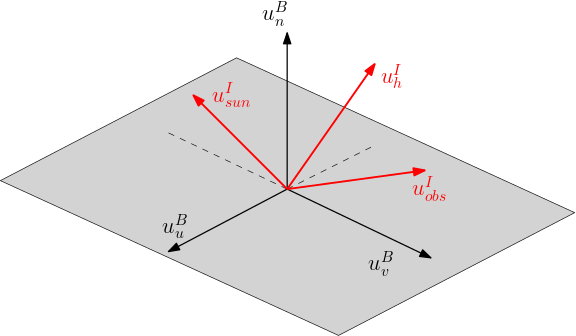
\includegraphics[width=0.6\textwidth]{Figures/Geom_reflexion.png}
    \caption{Geometría de la reflexión}
    \label{fig:geom-reflex}
\end{figure}

In addition, in order to obtain the value of the apparent magnitude, it is needed to model the light curve. This entails having the vectors that define the target's facets in inertial coordinates, denoted by the superscript $I$. To achieve this, the attitude matrix defined by the quaternion associated with the satellite at each moment is employed:

\begin{equation}
\mathbf{u}_k^b = A(\mathbf{q_I^B})\mathbf{u}_k^I, \quad k = u, v, n,
\end{equation}

Simultaneously, it is fundamental to determine the vector representing the sun with respect to the target, $\mathbf{u}_{\text{sun}}^I$, and the vector depicting the target's orientation concerning the observer, $\mathbf{u}_{\text{obs}}^I$.

With the directions of the reflected light with respect to the inertial frame defined, it is now possible to ascertain the variables that the observer will be able to see.

\subsection{Observation model}
Consider that the observing satellite is in a position $\boldsymbol{r_{obs}}$, capable of measuring the azimuth and elevation of the target, $\boldsymbol{r_{RSO}}$. The pointing vector from the observer to the RSO is defined as:
\begin{equation}
    \boldsymbol{d}=\boldsymbol{r_{RSO}}-\boldsymbol{r_{obs}}
\end{equation}

Furthermore, assume that the observer's sensors can measure the magnitude of the reflected light, modeled using the Phong light diffusion model \cite{Phong}, based on the Bidirectional Reflectance Distribution Function (BDRF). In this reference, the authors decompose the BDRF into a specular part (with a preferred direction), $\rho_{spec}$, and a diffuse part, $\rho_{diff}$:
\begin{equation}
    \rho_{tot}(i)=\rho_{spec}(i)+\rho_{diff}(i)\quad i=1...n_c,
\end{equation}
where $n_c$ is the number of facets of the RSO. Assuming flat faces, the specular part of the distribution results in:
\begin{equation}
    \rho_{\mathrm{spec}}(i)=C_{\mathrm{spec}}\frac{(\mathbf{u_{obs}^{I}}\cdot\mathbf{u_{spec}^{I}})}{(\mathbf{u_{sun}^{I}}\cdot\mathbf{u_{n}^{I}})},
\end{equation}
where the vector $\mathbf{u_{spec}^{I}}$ is the preferred direction of specular reflection, defined as $\mathbf{u_{spec}^{I}}=2(\mathbf{u_{n}^{I}}\cdot\mathbf{u_{sun}^{I}})\mathbf{u_{n}^{I}-u_{sun}^{I}}$. On the other hand, the diffuse term results in:
\begin{equation}
    \rho_{diff}(i)=\frac{C_{diff}}{\pi}.
\end{equation}
where $C_{spec}$ and $C_{diff}$ are reflection coefficients dependent on the RSO's surface material.

As the apparent magnitude is the measure reaching the observer's sensors of the light reflected by the RSO, the first step is to calculate the fraction of (visible) light reaching the RSO:
\begin{equation}
    F_{\mathrm{sun}}(i)=\Phi_{\mathrm{sun,vis}}\rho_{\mathrm{total}}(i)(\mathbf{u}_{n}^{I}(i)\cdot\mathbf{u}_{\mathrm{sun}}^{I}),
\end{equation}
where $\Phi_{\mathrm{sun,vis}}$ is the power per unit area received by an object illuminated by sunlight. Only a fraction of the light reflected by the RSO is visible to the observer:
\begin{equation}
    F_{\mathrm{obs}}(i)=\frac{F_{\mathrm{sun}}(i)\mathcal{A}(i)(\mathbf{u}_{n}^{I}(i)\cdot\mathbf{u}_{\mathrm{obs}}^{I})}{\|\mathbf{d}^{I}\|^2}.
\end{equation}

Finally, the apparent magnitude is given by a sum of the fraction of light the observer receives from each of the facets  the RSO :
\begin{equation}
    m_{\mathrm{app}}=-26.7-2.5\log_{10}\left|\sum_{i=1}^{N_{F}}\frac{F_{\mathrm{obs}}(i)}{\Phi_{\mathrm{sun,vis}}}\right|.
    \label{eqn:mapp}
\end{equation}

Note that, for the RSO to reflect light, it must be illuminated by sunlight, meaning that the periods of eclipse need to be restricted. Furthermore, if either the angle between the surface normal and the observer or the angle between the surface normal and the Sun direction is greater than $\pi/2$ the observer will not receive any light from this surface. 

These calculations have been implemented in the simulator through the \textit{magnitude\_apparent.m} function, presented below:

% \begin{lstlisting}[language=Matlab, caption= Excerpt of function \textit{magnitude\_apparent.m}.]
   
%     function mapp = magnitude_apparent1(ro_vir, rt, rsun, qt, SO)
%     phi_sun_vis = 455;
%     alpha = 1;
%     Rt=6378e3;

%     % Number of observers
%     n_observers = size(ro_vir, 1);

%     for j = 1:n_observers
       
%         % Vector from observer to target
%         d = rt' - ro_vir(j, :);
%         % Normalize vectors
%         u_obs_I = normr(-d);
%         u_sun_I = normr(rsun - rt');

%         % Check if the target is in eclipse
%         angle_target_sun = real(acos(dot(rt, rsun)/(norm(rsun) * norm (rt))));
%         eclipse_angle = asin(Rt/norm(rt));
%         if angle_target_sun > (pi-eclipse_angle) || (angle_target_sun < (eclipse_angle + pi) && angle_target_sun > (pi-eclipse_angle))
%             % Target is in eclipse, set solar flux to zero
%             fobs = 0;
            
%         else
%             % Initialize apparent magnitude
%             fobs = 0;

%             % Loop over surface elements
%             for k = 1:6
%                 % Rotate surface normal to inertial frame
%                 u_n_I = (quat2rotm(qt') * SO.Normals(k, :)')';

%                 % Compute angles between surface normal, observer's direction, and Sun direction
%                 angle_obs = acos(dot(u_n_I, u_obs_I));
%                 angle_sun = acos(dot(u_n_I, u_sun_I));

%                 % Check if either angle is greater than pi/2
% %                 if (angle_obs > pi/2 && angle_obs < 3*pi/2) || (angle_sun > pi/2 && angle_sun < 3*pi/2)
% %                     % No light reflected toward the observer
% %                     fsun = 0;
% %                     break
% %                 else
%                     % Compute reflected and diffuse components
%                     u_esp_I = 2 * dot(u_n_I, u_sun_I) * u_n_I - u_sun_I;
%                     rho_esp = SO.Cesp(k) * dot(u_obs_I, u_esp_I)^alpha / dot(u_sun_I, u_n_I);
%                     rho_dif = SO.Cdif(k) / pi;

%                     % Compute solar flux
%                     fsun = phi_sun_vis * (rho_dif + rho_esp) * dot(u_n_I, u_sun_I);
% %                 end

%                 % Accumulate flux from each surface element
%                 fobs = fsun * SO.Areas(k) * dot(u_n_I, u_obs_I) / norm(d)^2 + fobs;
%             end
%         end

%         % Calculate apparent magnitude for the observer
%         mapp(j) = -26.7 - 2.5 * log10(fobs / phi_sun_vis);
%     end
% end
% \end{lstlisting}

From this function, a significant portion of the results presented in Section \ref{s: resultados} has been derived. The \textit{magnitude\_apparent.m} function, described earlier, has played an important role in computing various outcomes that contribute to the findings detailed in the subsequent section. 


\newpage
\section{Analysis and results}\label{s: resultados}
Based on the enhancements made to the simulator and the new implementations in the photometry module, results have been extracted that must be carefully analyzed for the ongoing improvement of the simulator in terms of precision.

\subsection{Visibility sphere radius analysis}
Primarily, the \textit{magnitude\_apparent.m} function has been employed to conduct a comprehensive sweep considering the size of the debris (RSO) and the distance $\mathbf{d}$ between the observer and the RSO. The objective is to determine the radius of the observer's visibility sphere, a critical parameter in understanding the simulation outcomes and optimizing precision. 

To achieve this, multiple simulations have been conducted by placing the observer in a fixed circular orbit with orbital parameters detailed in \autoref{tab:paramsobs}, which have been chosen to manage a relative position between the observer, the sun and the RSO that allows the visibility of the RSO. Additionally, various RSOs of different sizes have been generated, each placed in circular orbits within the same orbital plane while varying the semi-major axis of their orbits. However, as the attitude of the RSOs is generated randomly, several simulations were conducted for each combination of distance and RSO size, to get the average visibility in each case.

 
\begin{table}[H]
    \centering
    \caption{Orbital parameters of the observer's orbit.}
    \begin{tabular}{ccc}
    \toprule
    $\boldsymbol{a}$ [km] & $\boldsymbol{e}$ [-] & $\boldsymbol{i}$ [$^\circ$] \\
    \midrule
      6878  & 0  & 0.6 \\
    \bottomrule
    \end{tabular}
    \label{tab:paramsobs}
\end{table}
    

In Figures \ref{fig:mapp-distance} and \ref{fig:mapp-size}, the dependencies among the size, distance, and apparent magnitude of the RSO are illustrated. These figures depict how the apparent magnitude varies concerning the reduction in the RSO size and/or an increase in the distance between the RSO and the observer. It is observed that the magnitude increases (indicating reduced visibility\footnote{It is noteworthy that as defined in \autoref{eqn:mapp}, the more negative the magnitude, the more visible the RSO is to the observer.}) with a decrease in the RSO size and/or an increase in the separation between the RSO and the observer.

\begin{figure}[H]
    \centering
    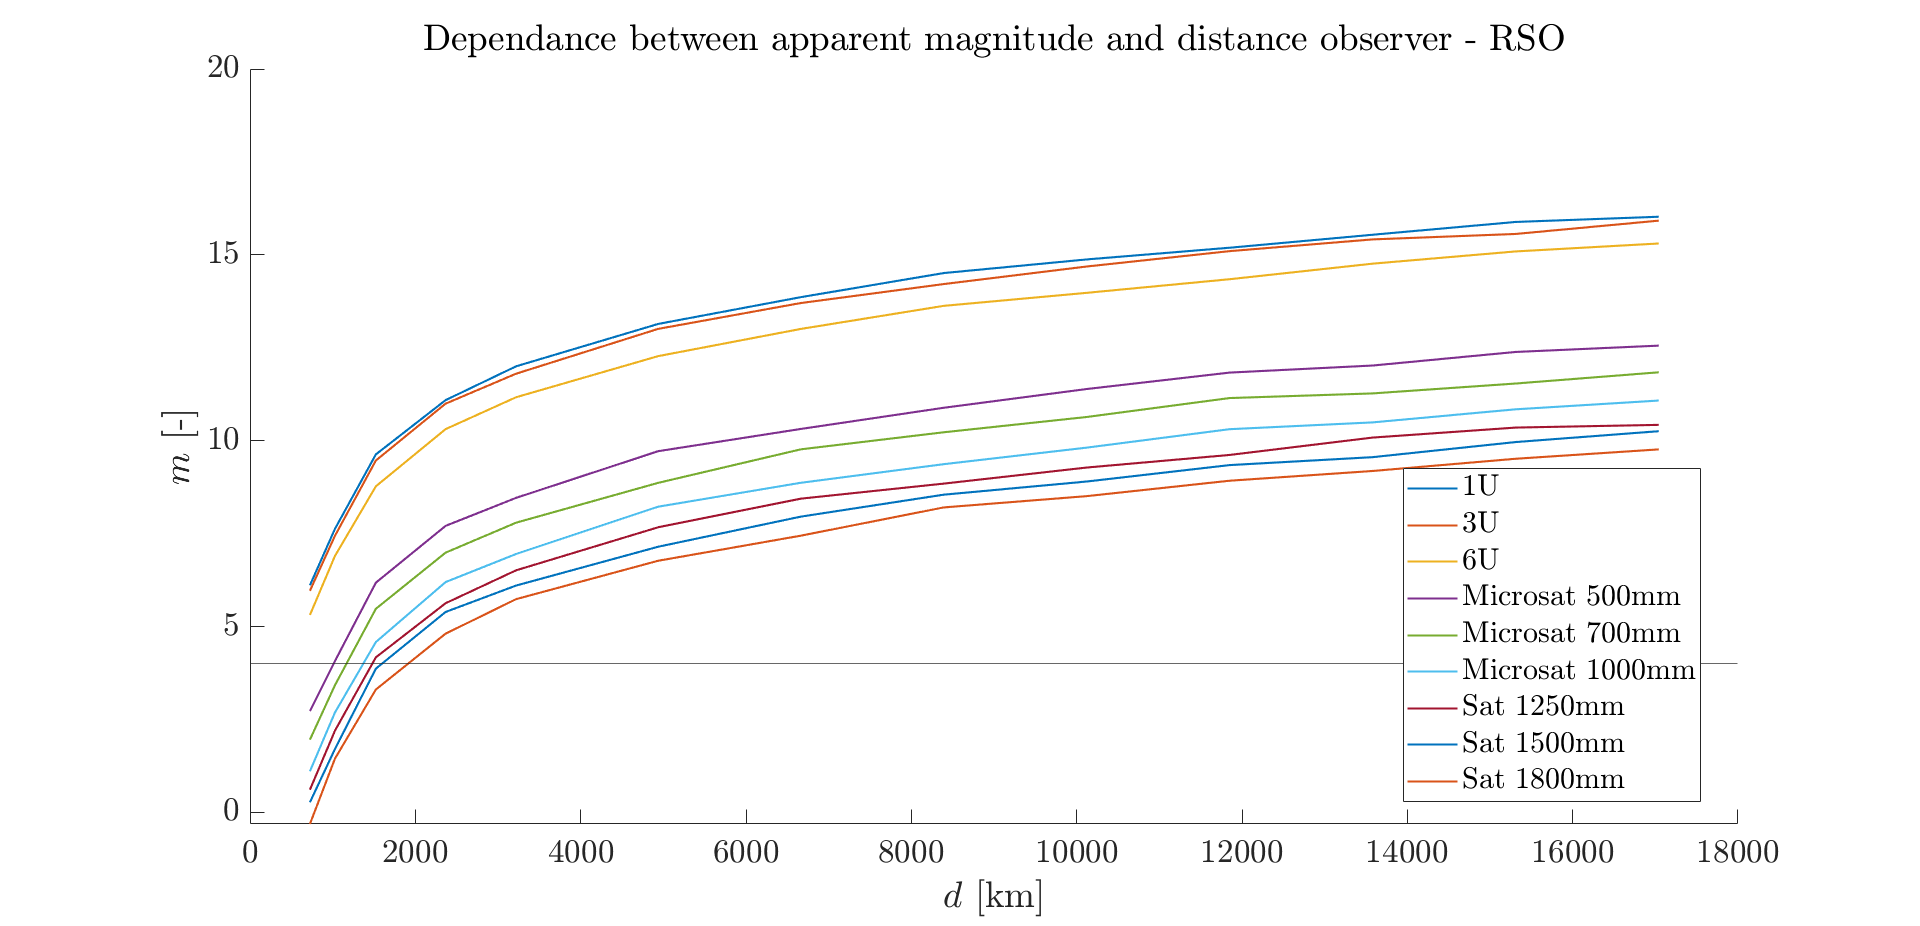
\includegraphics[width=\textwidth]{Figures/mapp-distance.png}
    \caption{}
    \label{fig:mapp-distance}
\end{figure}
\begin{figure}[H]
    \centering
    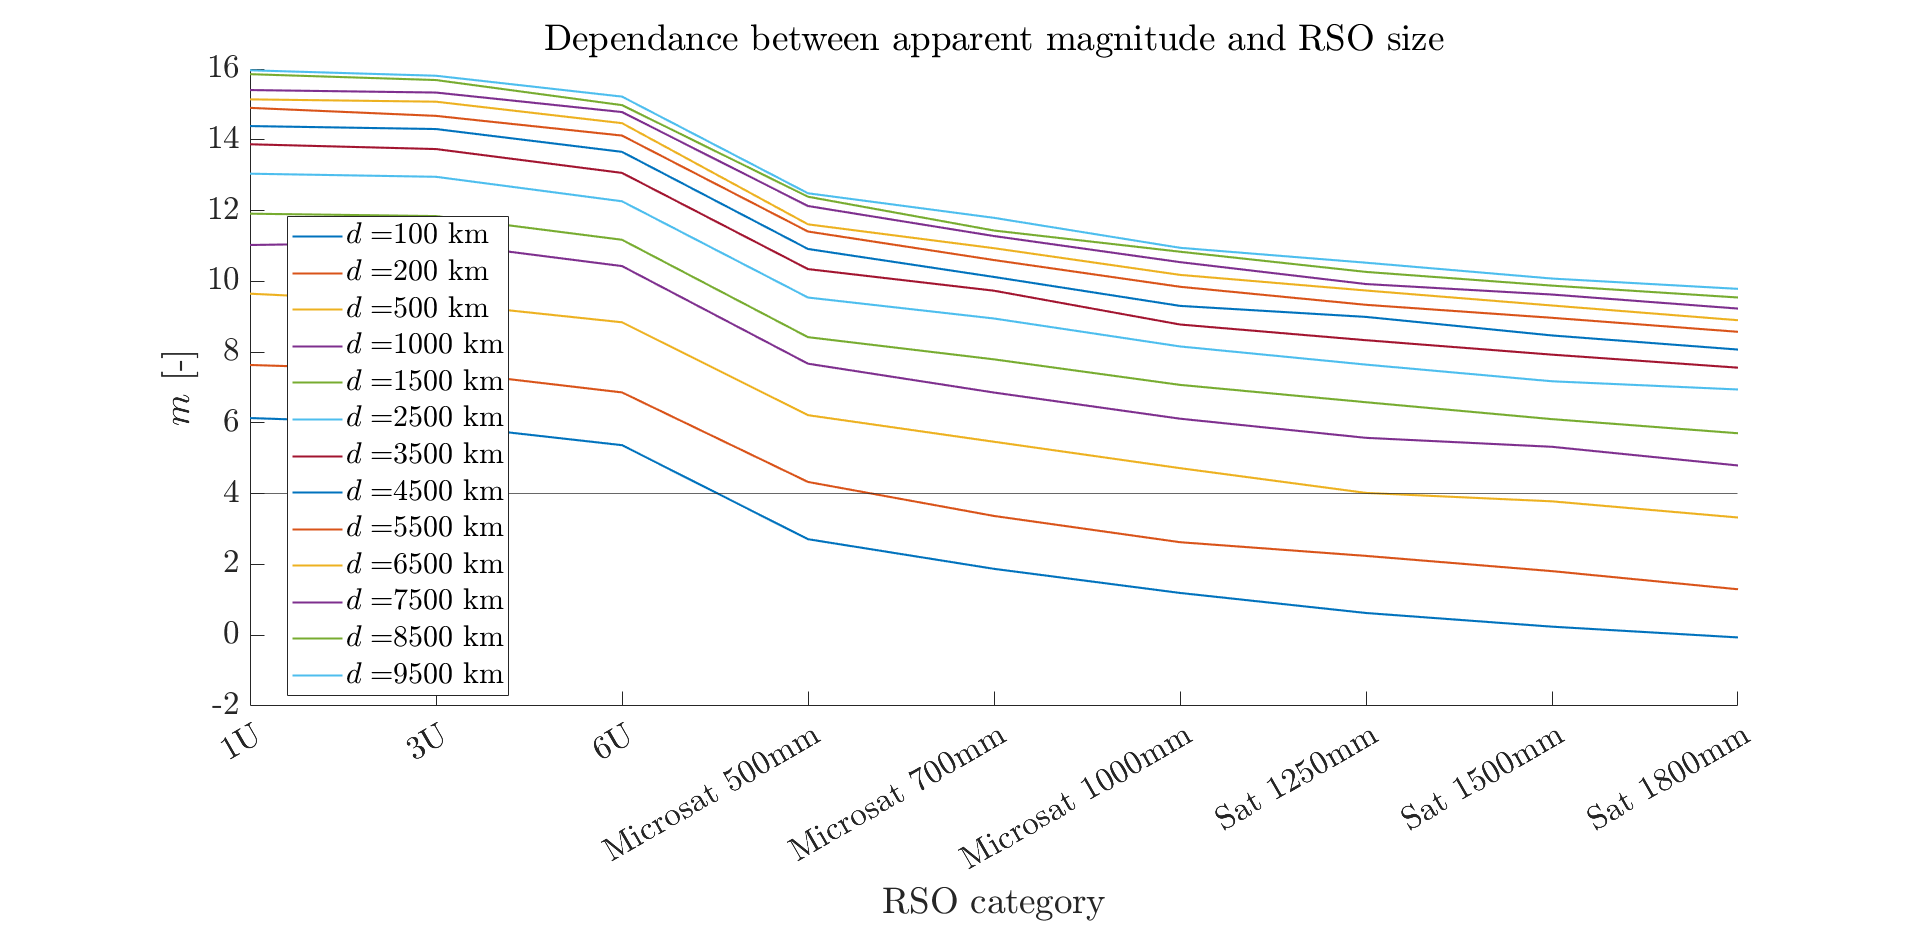
\includegraphics[width=\textwidth]{Figures/size-mapp.png}
    \caption{}
    \label{fig:mapp-size}
\end{figure} 

The apparent magnitude that the observer is able to perceive is constrained by the optical sensors employed, which will depend on factors such as the mission budget, the number of observers, and the desired constellation type. Initially, the plan is to utilize a constellation of cubesats equipped with basic tracking cameras. Following the guidelines from \cite{limmapp}, a visibility threshold has been set at $m=4$.

Returning to the examination of the previous figures, this constraint on the apparent magnitude that the observer can perceive limits a range of distances and sizes of RSOs that the satellite will be able to detect. Thus, it has been established that the observer-RSO limit distance for the sensors to detect the RSO is around $d=1000 \, \text{km}$.

\subsection{Observation windows}
On the other hand, to comprehend the influence of the Sun's position on the fraction of reflected light reaching the observer, another scan has been conducted. In this case, the observer (again with the orbital parameters outlined in \autoref{tab:paramsobs}) and the RSO are kept fixed, while the sun's location (in Earth inertial axes) is varied over the course of a year. The outcome of this procedure is depicted in \autoref{fig:angle-mapp}.

This figure shows the relation between the apparent magnitude of the RSO and $\theta$ (defined as the angle formed by the position vector of the RSO $\boldsymbol{r_{RSO}}$ and the Sun $\boldsymbol{r_{Sun}}$projeted into the ecuatorial plane).
\begin{figure}[H]
    \centering
    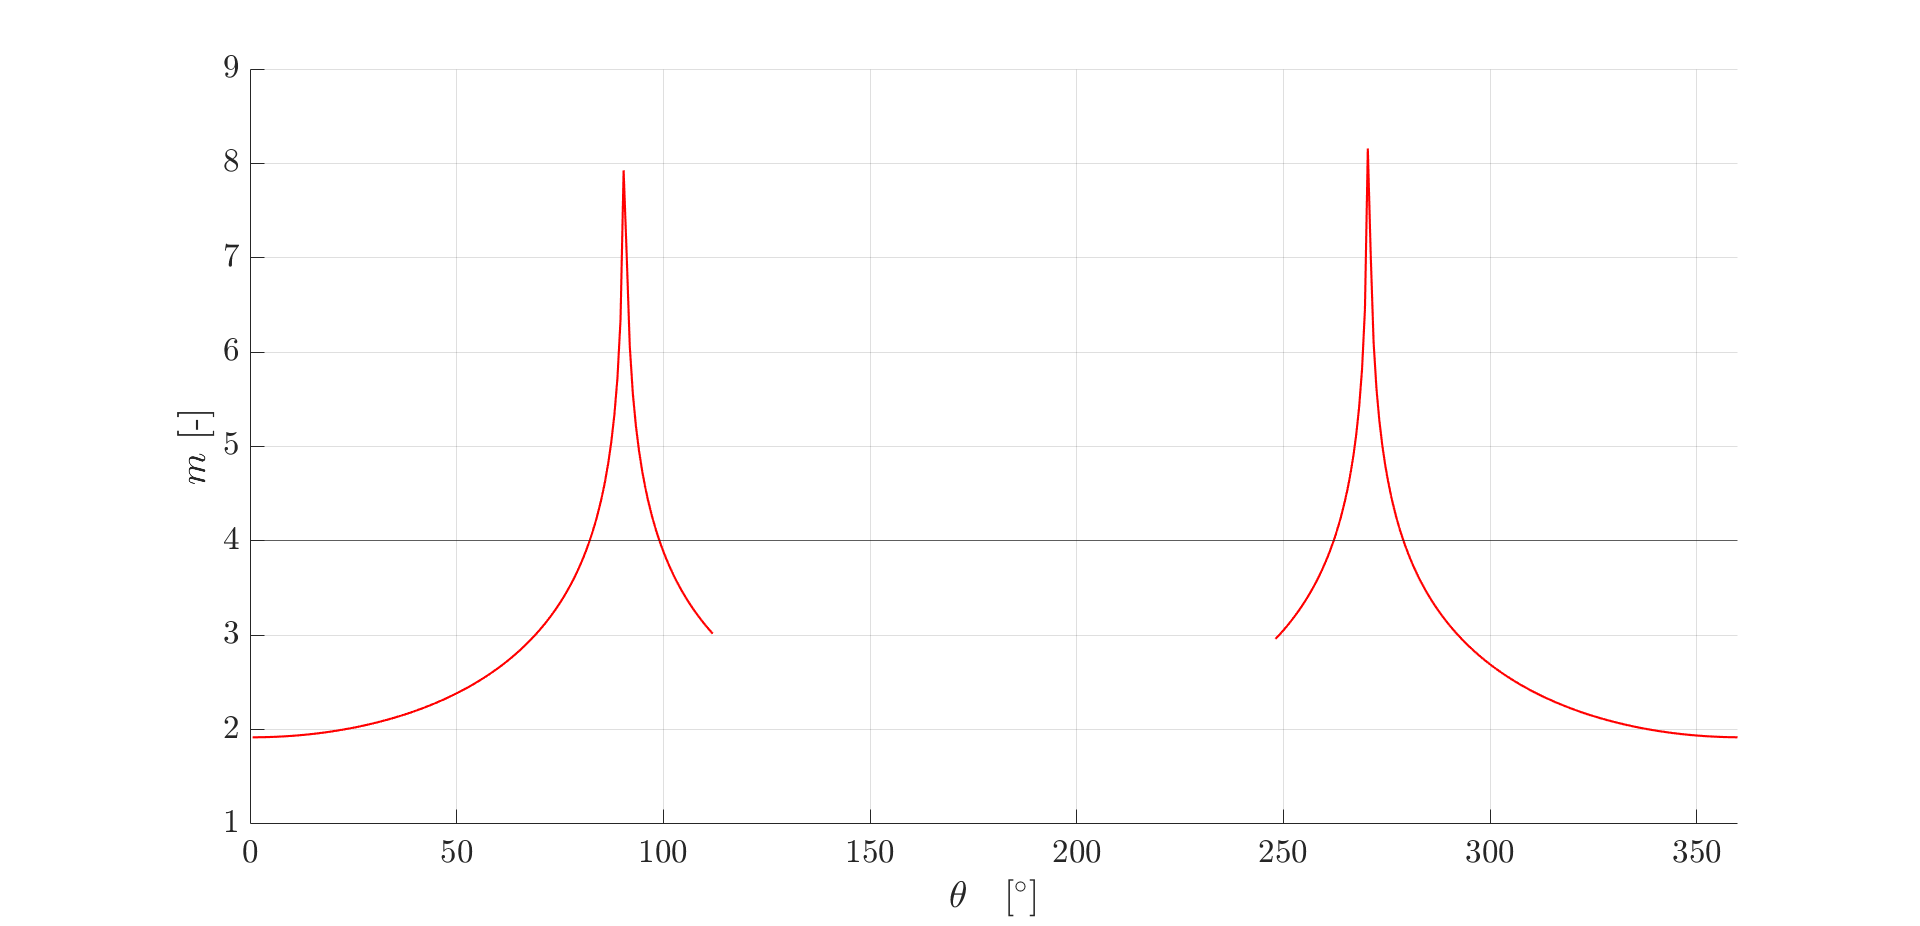
\includegraphics[width=\textwidth]{Figures/anglesunRSO-mapp.png}
    \caption{Dependance of the apparent magnitude $m$ with the position of the Sun relative to the observer.}
    \label{fig:angle-mapp}
\end{figure}

Within the figure, it is evident that the optimal solar position occurs when $\theta$ is in close proximity to zero. However, it is fundamental to note a potential intricacy in the case of an Above-the-Horizon (ATH) coverage. Specifically, if the target aligns precisely with the sun, the resulting light curve from the target may be entirely eclipsed by the incoming sunlight. Nonetheless, for Below-the-Horizon (BTH) orbits and/or distinct inclinations, the presented outcome within this graph remains accurate. As this angle is not an input to the program, it must be translated to the date it corresponds, which can be seen in \autoref{fig:date-mapp}, where the date-defined observation window can be seen. 
\begin{figure}[H]
    \centering
    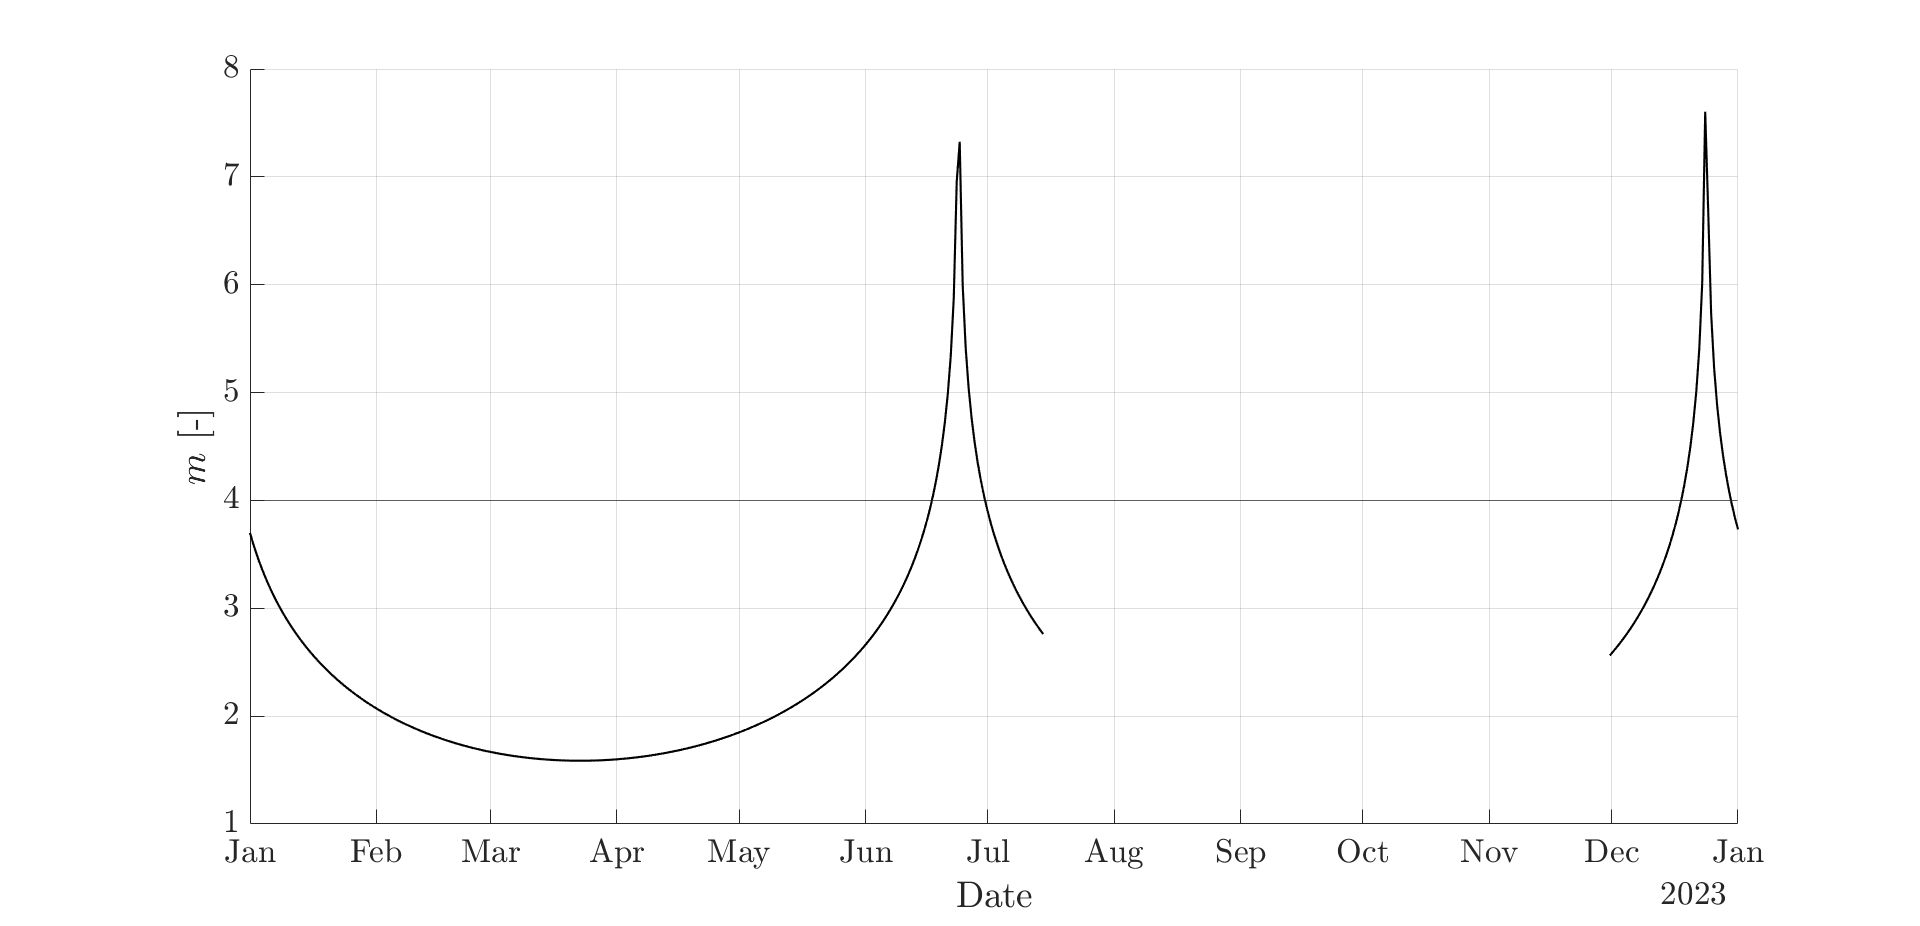
\includegraphics[width=\textwidth]{Figures/date-mapp.png}
    \caption{Dependance of the apparent magnitude $m$ with the position of the Sun in terms of date.}
    \label{fig:date-mapp}
\end{figure}

\begin{table}[H]
    \centering
    \caption{Observation window}
    \begin{tabular}{ccc}
    \toprule
     & \textbf{Start} & \textbf{End} \\
    \midrule
      $\boldsymbol{\theta}$ [$^\circ$]  & -60 & 60 \\
      \textbf{Date} & 1 January 2023 & 16 June 2023 \\
    \bottomrule
    \end{tabular}
    \label{tab:ventanas}
\end{table}

Based on these outcomes, observation windows have been delineated to subsequently conduct simulations in which the RSO falls within the field of view of the observer. 

With the information of these findings, observation windows have been meticulously defined to conduct subsequent simulations where the RSO resides within the visibility sphere of the observer. It is noteworthy that, for this parameter sweep, a distance of 300 km between the RSO and the observer has been considered, incorporating BTH coverage, and using a square-shaped satellite with a side length of 1 m.

\subsection{Visibility times}
Subsequently, multiple simulations have been executed with varying numbers of observers to assess visibility durations. For this purpose, the RSO has been fixed in an orbit with parameters outlined in \autoref{tab:paramstarget}, within the launch windows specified in \autoref{tab:ventanas}. It is essential to note that while the observation window scan was conducted for a satellite with a side length of 1 m, in this scenario, to ensure robust visibility regardless of the RSO's attitude, simulations have been conducted with a satellite measuring 1.5 m in side length.
\begin{table}[H]
    \centering
    \caption{Orbital parameters of the RSO's orbit.}
    \begin{tabular}{ccc}
    \toprule
    \textbf{$a$ [km]} & \textbf{$e$ [-]} & \textbf{$i$ [$^\circ$]} \\
    \midrule
    6878 & 0 & 0.6 \\
    \bottomrule
    \end{tabular}
    \label{tab:paramstarget}
\end{table}

The obtained observation times have been illustrated in \autoref{fig:T-tvis} and dimensionless representations, relative to the total simulation time, are presented in \autoref{fig:percentages}. This approach provides a clear visualization of the fraction of the orbit covered by the observer.

\begin{figure}[H]
    \centering
    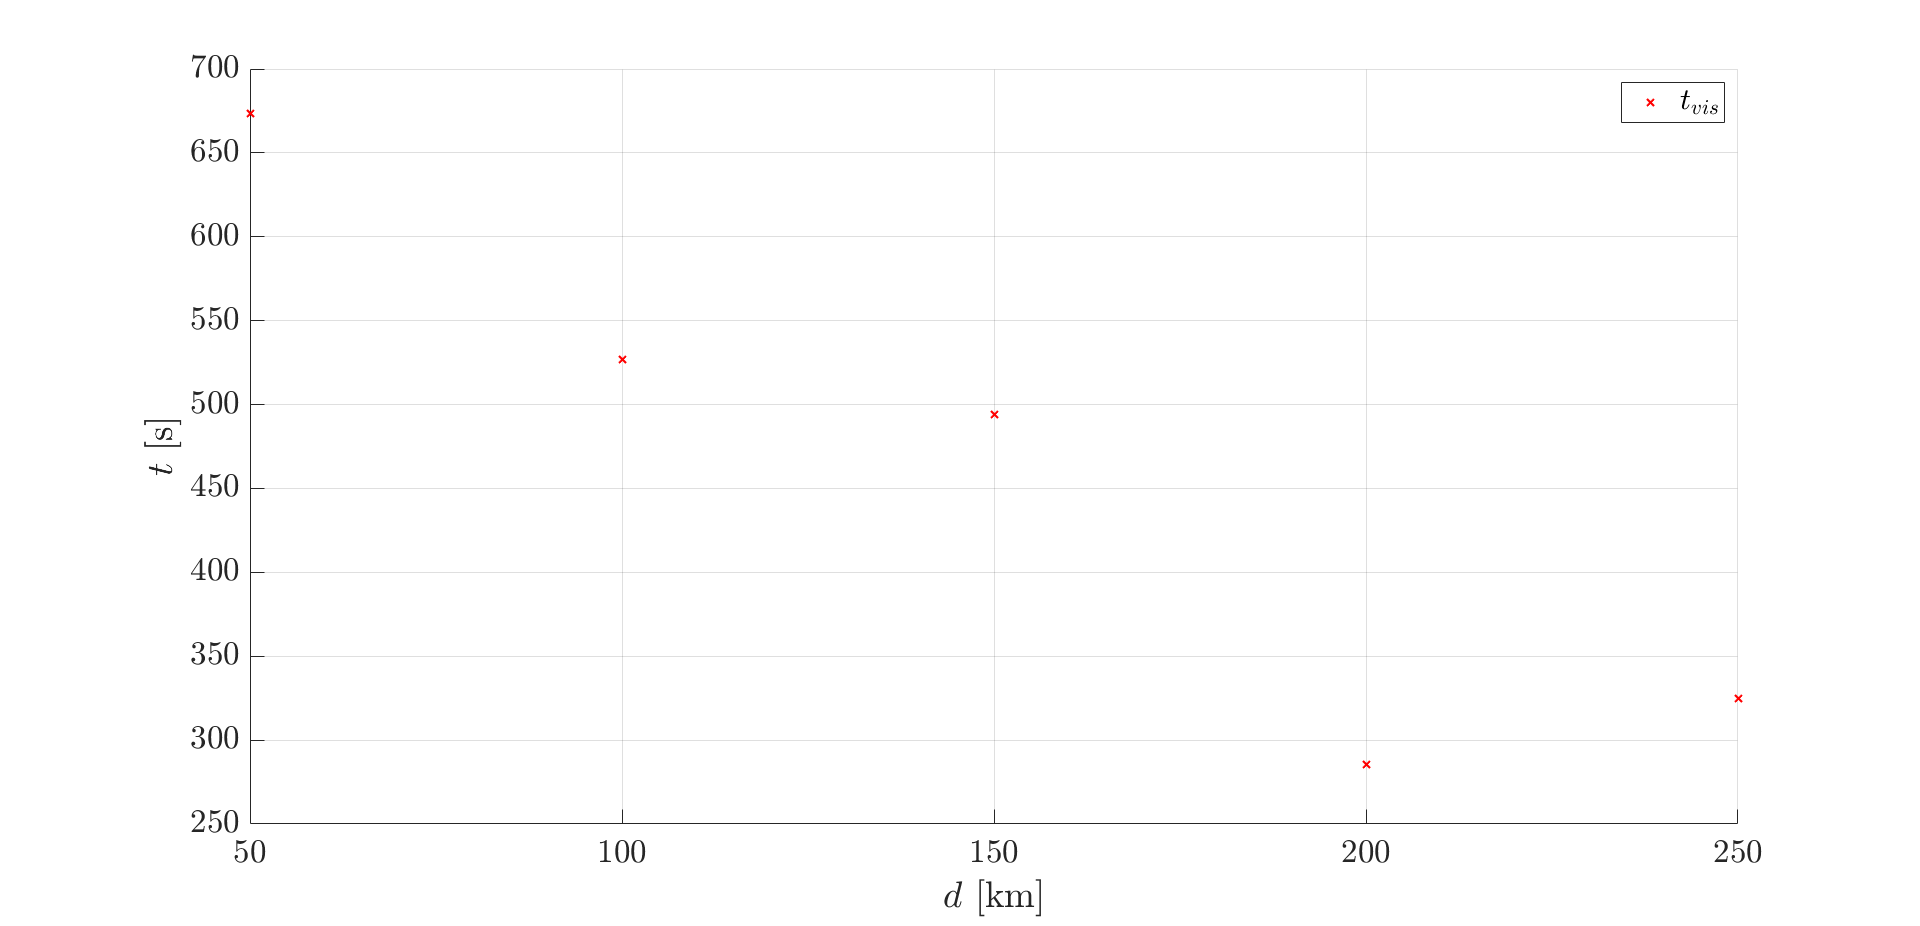
\includegraphics[width=\textwidth]{Figures/T-tvis.png}
    \caption{Dependance of the observation time with the distance between the observer and the RSO}
    \label{fig:T-tvis}
\end{figure}

\begin{figure}[H]
    \centering
    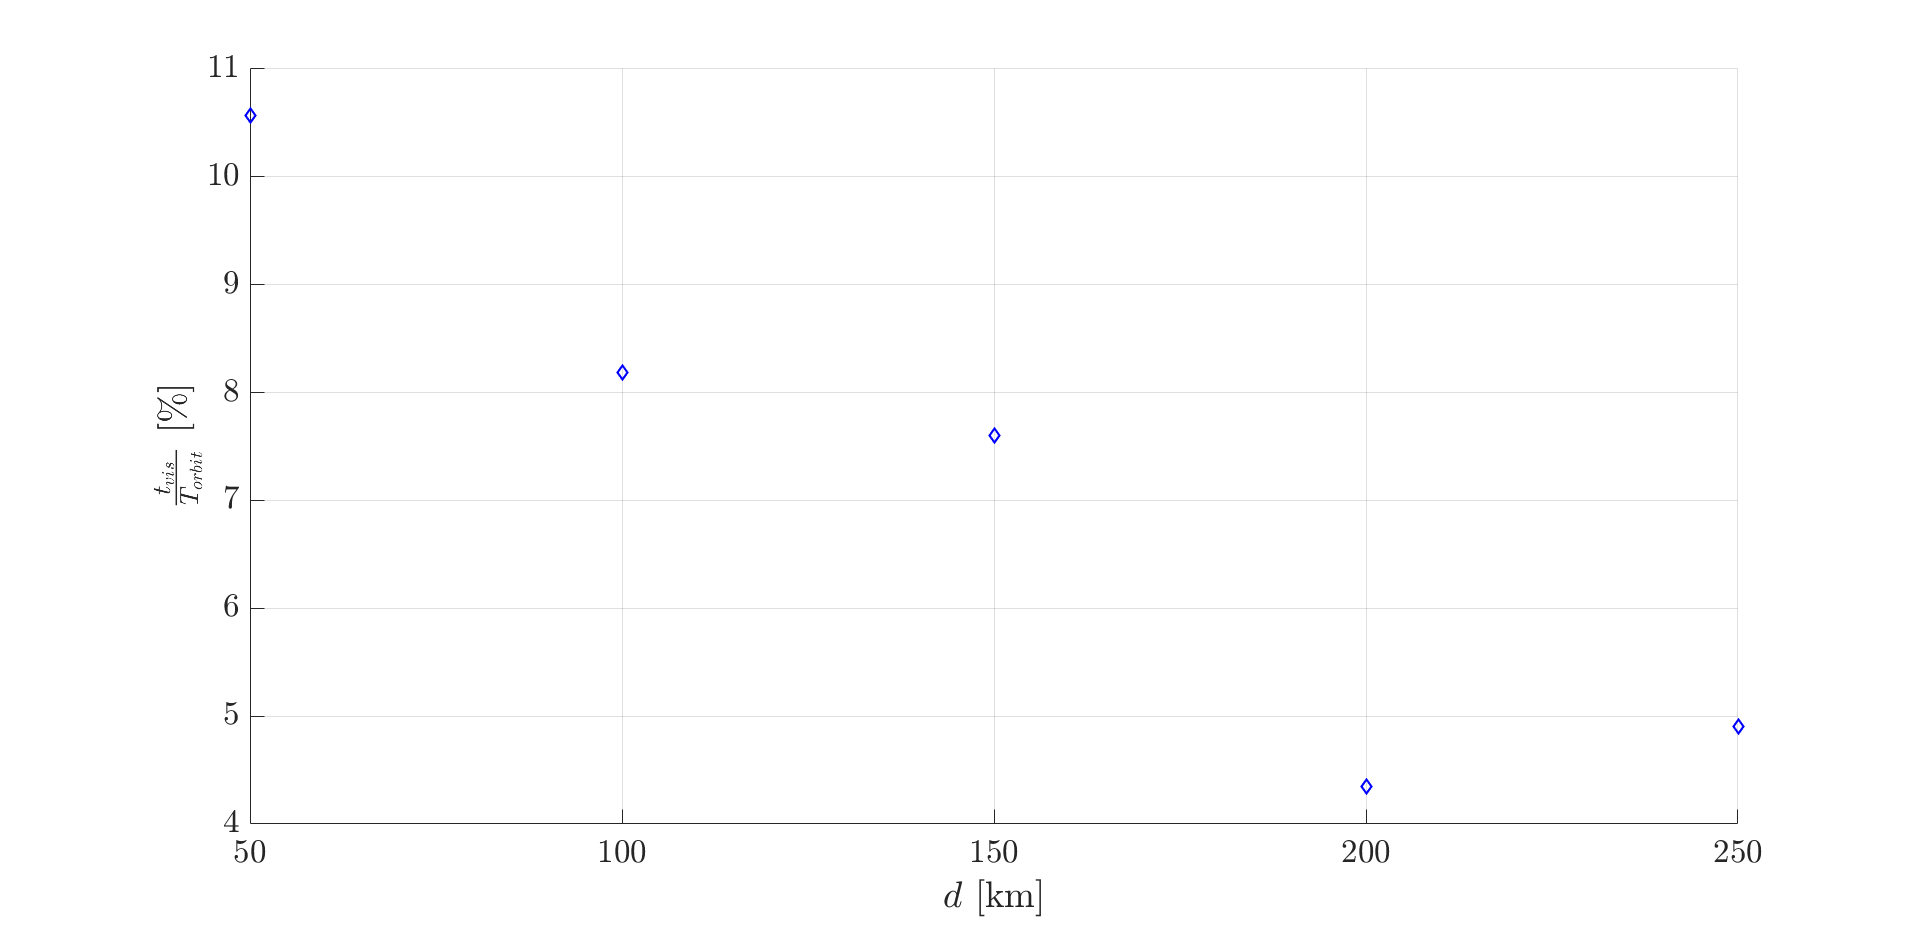
\includegraphics[width=\textwidth]{Figures/percentage-orbit.png}
    \caption{Relation between the percentage of orbit visible and the distance between the observer and the RSO}
    \label{fig:percentages}
\end{figure}




\newpage
\clearpage
\bibliographystyle{plain}
\bibliography{bibliography.bib}
\newpage
\clearpage

% \appendix
% \input{Appendix}

\end{document}



